\documentclass[]{beamer}

\usetheme{metropolis}
\metroset{progressbar=frametitle}
\usefonttheme[onlymath]{serif}

\usepackage[none]{hyphenat}
\usepackage{hyperref}
\usepackage{amsmath}
\usepackage{amsfonts}
\usepackage{amssymb}
\usepackage[normalem]{ulem}
\usepackage{graphicx}
\usepackage{tikz}
\usepackage{minted}
\author{Maxim Borisyak, Claude Code, Andrey Ustyuzhanin}
\institute{Constructor University Bremen}
\usepackage{booktabs}




\begin{document}



\title{Scientific Integrity and Research Misconduct}

\begin{frame}[plain]
\titlepage
\end{frame}

\section{Science as a Collective Enterprise}

\begin{frame}[fragile]
\frametitle{Scientific is Iterative}
Each result is an input to subsequent works:
\begin{itemize}
  \item cited as established fact in future introductions;
  \item reused as a baseline for comparison;
  \item built upon in methods, proofs, and datasets;
  \item research is planned based on prior results.
\end{itemize}

\begin{align*}
\text{Integrity violation}\quad &\Longrightarrow \quad \text{systematic pollution};\\
    &\Longrightarrow \quad \text{misguided future research};\\
    &\Longrightarrow \quad \text{wasted resources and time}.
\end{align*}

\end{frame}

\begin{frame}[fragile]
\frametitle{The Spectrum of Misconduct}
{\footnotesize
\begin{tabular}{p{3.5cm} p{6.5cm}}
\toprule
\textbf{Category} & \textbf{Description} \\
\midrule
Honest error & Mistakes in analysis, code, misinterpretation \\
\addlinespace
Questionable Research Practices (QRPs) & Decisions that inflate apparent evidence without outright fabrication \\
\addlinespace
Research misconduct (FFP) & Deliberate fabrication, falsification or plagiarism \\
\bottomrule
\end{tabular}
}

\end{frame}

\section{Fabrication and Falsification}

\begin{frame}[fragile]
\frametitle{Fabrication}
\textbf{Fabrication}: reporting data that were never collected.

Cases:
\begin{itemize}
  \item \textbf{Hwang Woo-suk} (2004): fabricated human stem cell lines; two \textit{Science} papers retracted;
  \item \textbf{Diederik Stapel} (2011): fabricated datasets for 55+ psychology papers;
  \item \textbf{Eric Poehlman} (2005): first US academic imprisoned for research fraud.
\end{itemize}

\end{frame}

\begin{frame}[fragile]
\frametitle{Falsification}
\textbf{Falsification}: altering data, images, or analyses to misrepresent reality.

Cases:
\begin{itemize}
  \item \textbf{Jan Hendrik Schön} (2002): reused figures across 16 papers in \textit{Science} and \textit{Nature}; identical noise patterns in independent experiments.
\end{itemize}

\end{frame}

\begin{frame}[fragile]
\frametitle{Plagiarism}
\textbf{Plagiarism}: presenting others' intellectual work as one's own.

Forms:
\begin{itemize}
  \item \textbf{verbatim copying}: reproducing text without proper attribution;
  \item \textbf{paraphrasing}: rewording ideas without citation;
  \item \textbf{idea theft}: using results from peer review or collaboration;
  \item \textbf{self-plagiarism}: republishing prior work without disclosure.
\end{itemize}

\end{frame}

\begin{frame}[fragile]
\frametitle{Plagiarism}
\textbf{Copying via LLMs}: using text produced by LLMs:
\begin{itemize}
  \item LLMs can reproduce many texts almost verbatum (Ahmed~et~al.~2025, Huang~et~al.~2026):
  \item studies strongly suggests that LLM output is an amalgamation of others works;
  \item naturally, without attribution.
\end{itemize}

\end{frame}

\begin{frame}[fragile]
\frametitle{Consequences}
\begin{itemize}
  \item retraction --- often years after publication;
  \item cascade retractions of papers that cited the work;
  \item loss of employment, funding, academic standing;
  \item criminal prosecution in extreme cases (Poehlman).
\end{itemize}

\textbf{Retraction half-life} in biomedicine: $\approx 10$ years.

\end{frame}

\section{Statistical Malpractice}

\begin{frame}[fragile]
\frametitle{The Logic of Hypothesis Testing}
A frequentist test controls the \textbf{false positive rate}:
$$P(\text{reject } H_0 \mid H_0 \text{ true}) = \alpha$$

This holds only if:
\begin{enumerate}
  \item hypothesis fixed before seeing data;
  \item test performed exactly once.
\end{enumerate}

Both assumptions are routinely violated.

\end{frame}

\begin{frame}[fragile]
\frametitle{The Multiple Comparisons Problem}
$k$ independent tests under $H_0$:
$$P(\text{at least one false positive}) = 1 - (1-\alpha)^k$$

\begin{itemize}
  \item $k = 1$, $\alpha = 0.05$: $P = 0.05$;
  \item $k = 20$, $\alpha = 0.05$: $P \approx 0.64$.
\end{itemize}

\end{frame}

\begin{frame}[fragile]
\frametitle{The Base Rate Fallacy}
$\alpha$ controls $P(\text{reject } H_0 \mid H_0 \text{ true})$, not $P(H_0 \text{ true} \mid \text{reject } H_0)$.

Researchers routinely conflate the two — this is the \textbf{base rate fallacy}:
\begin{itemize}
  \item $p < 0.05$ does \textbf{not} mean "5\% chance the null is true";
  \item the probability that a significant result reflects a real effect depends on the prior probability that $H_1$ is true.
\end{itemize}

\end{frame}

\begin{frame}[fragile]
\frametitle{Positive Predictive Value}
Let $\pi = P(H_1 \text{ true})$, $1 - \beta$ = power. Probability that a significant result is genuine:

$$\mathrm{PPV} = \frac{\pi(1-\beta)}{\pi(1-\beta) + (1-\pi)\alpha}$$

\begin{itemize}
  \item high power and high $\pi$ $\Rightarrow$ most significant results are real;
  \item low $\pi$ (exploratory research, many hypotheses) $\Rightarrow$ most are false positives, even at $\alpha = 0.05$.
\end{itemize}

\end{frame}

\begin{frame}[fragile]
\frametitle{Positive Predictive Value}
\begin{figure}
\centering
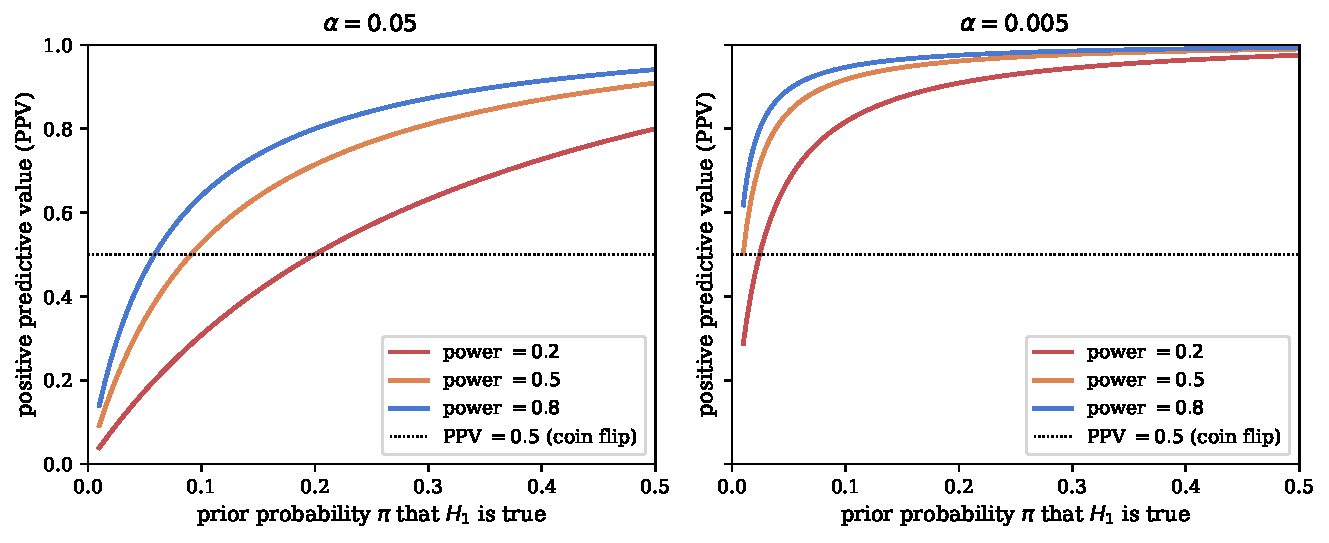
\includegraphics[width=0.95\textwidth]{imgs/ppv.pdf}
\end{figure}


{\small PPV vs.\ prior $\pi$ for three power levels. At $\alpha = 0.05$ (left), low-prior research produces mostly false positives even with 80\% power. Lowering $\alpha$ to 0.005 (right) substantially improves PPV.}

\end{frame}

\begin{frame}[fragile]
\frametitle{Why Most Published Research Findings Are False}
Ioannidis (2005) extended the PPV framework to account for bias:
\begin{itemize}
  \item in most fields, $\pi$ is small — hypotheses are cheap to generate;
  \item studies are underpowered ($1 - \beta \approx 0.2$--$0.5$);
  \item bias ($p$-hacking, QRPs) inflates the effective false positive rate beyond $\alpha$.
\end{itemize}

For many research areas, a significant result has less than even odds of reflecting a true effect.

\end{frame}

\begin{frame}[fragile]
\frametitle{p-Hacking in Practice}
\begin{figure}
\centering
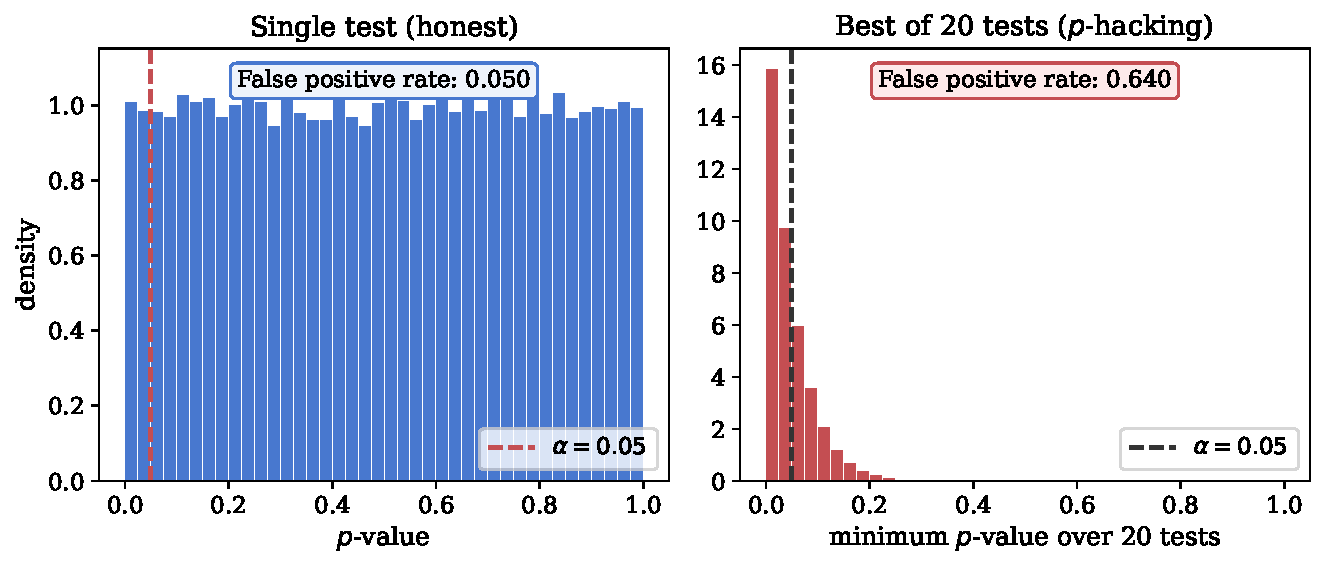
\includegraphics[width=0.95\textwidth]{imgs/phacking.pdf}
\end{figure}


{\small Single honest test: $p$-values uniform under the null (left). Best of 20 tests: false positive rate $\approx 64\%$ at nominal $\alpha = 0.05$ (right).}

\end{frame}

\begin{frame}[fragile]
\frametitle{Forms of p-Hacking}
Each decision below adds an implicit test:
\begin{itemize}
  \item \textbf{optional stopping}: collecting data until $p < 0.05$, then stop;
  \item \textbf{covariate fishing}: changing features based on their effect;
  \item \textbf{test switching}: choosing different tests;
  \item \textbf{outlier sculpting}: removing some outliers but not others:
\begin{itemize}
  \item the definition of outliers is often tied to the model;
\end{itemize}

  \item \textbf{outcome selection}: testing many hypotheses, reporting significant ones.
\end{itemize}

\end{frame}

\begin{frame}[fragile]
\frametitle{The Garden of Forking Paths}
Gelman \& Loken (2014): at every step (preprocessing, outlier criteria, covariates, outcome definition) multiple legitimate choices exist.

Selecting the path that "works" after seeing data $\rightarrow$ searching over all paths.

The resulting $p$-value is not calibrated to $\alpha$.

\end{frame}

\begin{frame}[fragile]
\frametitle{HARKing}
\textbf{HARKing} (Kerr, 1998): Hypothesising After Results are Known.

Mechanism:
\begin{enumerate}
  \item collect data; explore; find a pattern;
  \item rewrite the introduction as if the pattern was the original question.
\end{enumerate}

Effect: exploratory analysis presented as confirmatory $\Rightarrow$ evidential value destroyed.

\end{frame}

\begin{frame}[fragile]
\frametitle{Publication Bias}
\textbf{Publication bias}: positive results are published; null results are not.

Consequence: the literature overestimates effect sizes.

\textbf{Funnel plot}: studies scatter symmetrically around the true effect under no bias; publication bias creates visible asymmetry by removing small null-result studies.

\end{frame}

\begin{frame}[fragile]
\frametitle{Publication Bias}
\begin{figure}
\centering
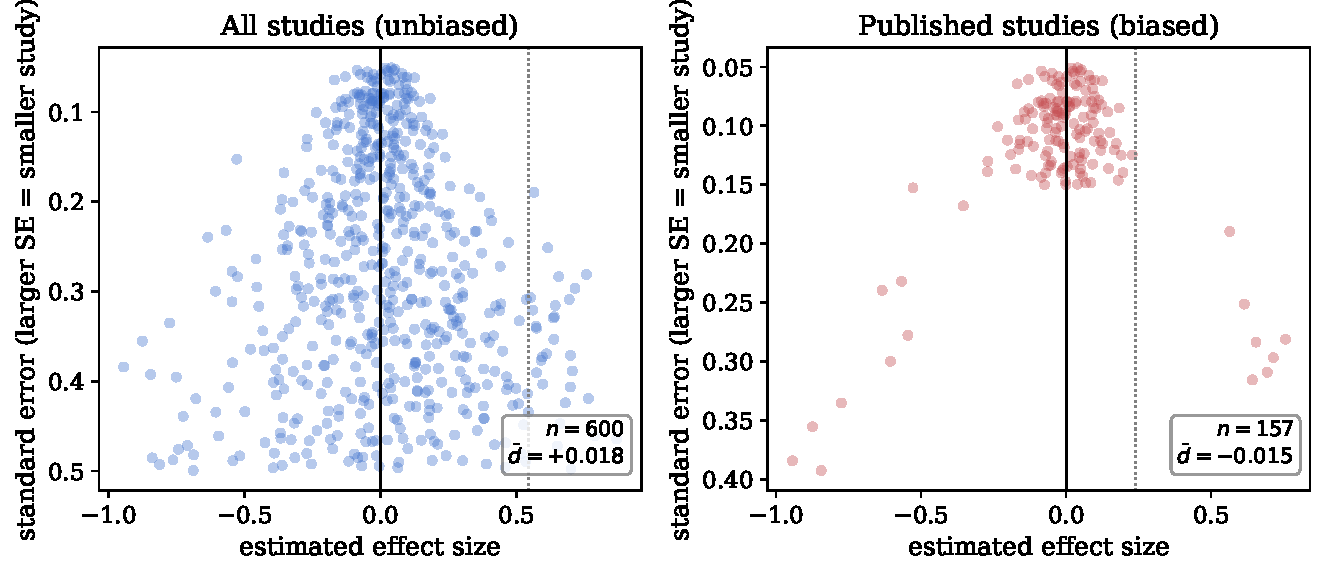
\includegraphics[width=0.95\textwidth]{imgs/funnel.pdf}
\end{figure}


{\small All studies (left) vs.\ published studies only (right). Small null-result studies are absent; mean reported effect $\bar{d}$ shifts away from zero.}

\end{frame}

\begin{frame}[fragile]
\frametitle{Selective Outcome Reporting}
\textbf{Outcome switching}: pre-register outcome $A$; report outcome $B$ when $A$ is non-significant.

\begin{itemize}
  \item Chan et al.\ (2004): 62\% of clinical trials changed, introduced, or omitted a primary outcome between registration and publication;
  \item pre-registration creates an auditable record that makes switching detectable.
\end{itemize}

\end{frame}

\section{Manipulation of Methodology}

\begin{frame}[fragile]
\frametitle{Inappropriate Baselines}
Reporting a method as better than an unfair comparison is not a contribution:
\begin{itemize}
  \item \textbf{weak baseline}: poorly tuned or outdated comparison method;
  \item \textbf{task asymmetry}: easier formulation for the baseline;
  \item \textbf{metric cherry-picking}: reporting the metric where the proposed method wins.
\end{itemize}

Tuning one method on validation data while using defaults for the baseline invalidates the comparison.

\end{frame}

\begin{frame}[fragile]
\frametitle{Cherry-Picking}
Selective presentation of evidence:
\begin{itemize}
  \item reporting only conditions where the method succeeds;
  \item excluding runs with inconvenient results;
  \item evaluating on a curated subset of the test set.
\end{itemize}

Statistical effect: identical to p-hacking — reported performance does not generalise.

\end{frame}

\begin{frame}[fragile]
\frametitle{Fabrication Detection: Benford's Law}
\textbf{Benford's Law}: naturally occurring data obey $P(\text{leading digit} = d) = \log_{10}(1 + 1/d)$.

\begin{figure}
\centering
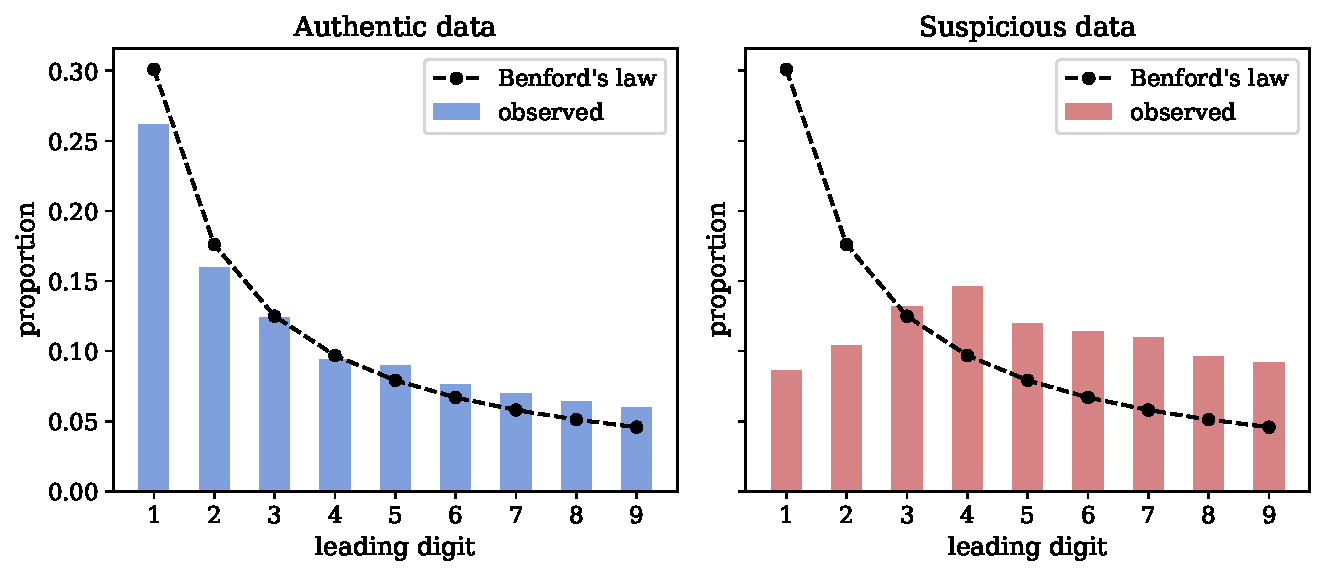
\includegraphics[width=0.95\textwidth]{imgs/benford.pdf}
\end{figure}


{\small Authentic data (left) conforms to Benford's Law. Fabricated data (right) deviates — humans generating numbers tend toward uniformity.}

\end{frame}

\begin{frame}[fragile]
\frametitle{Other Fabrication Signatures}
\begin{itemize}
  \item \textbf{terminal digit preference}: fabricated data clusters on 0 and 5;
  \item \textbf{GRIM test}: certain means are arithmetically impossible for integer-valued scales.
\end{itemize}

\end{frame}

\section{Graphical Misrepresentation}

\begin{frame}[fragile]
\frametitle{Truncated Y-Axis}
\begin{figure}
\centering
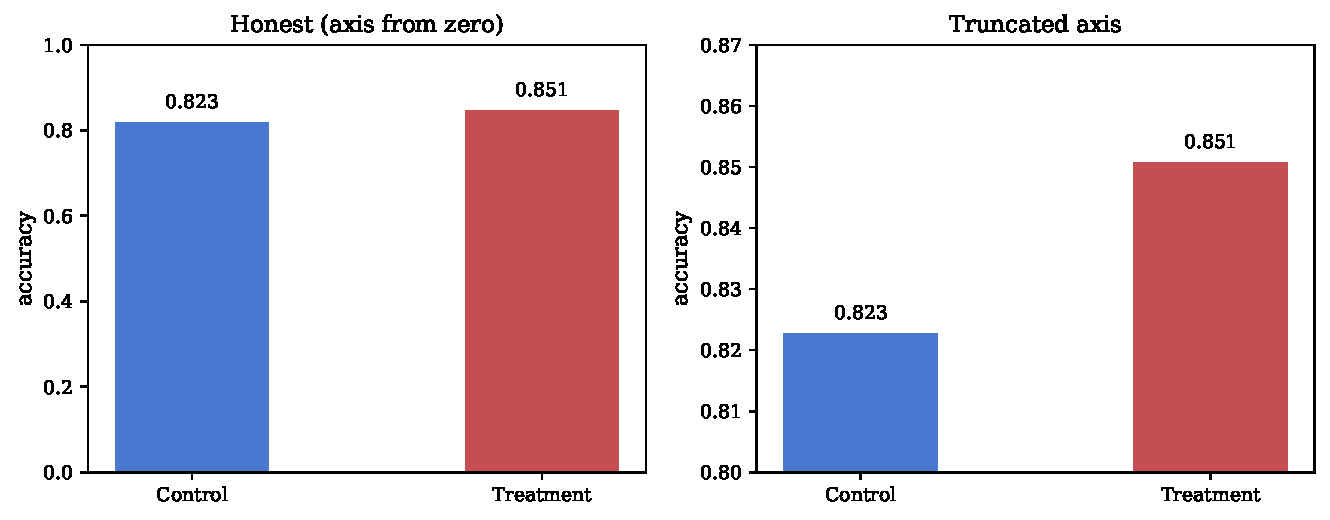
\includegraphics[width=0.95\textwidth]{imgs/truncated_axis.pdf}
\end{figure}


\end{frame}

\begin{frame}[fragile]
\frametitle{Cherry-Picking a Time Window}
\begin{figure}
\centering
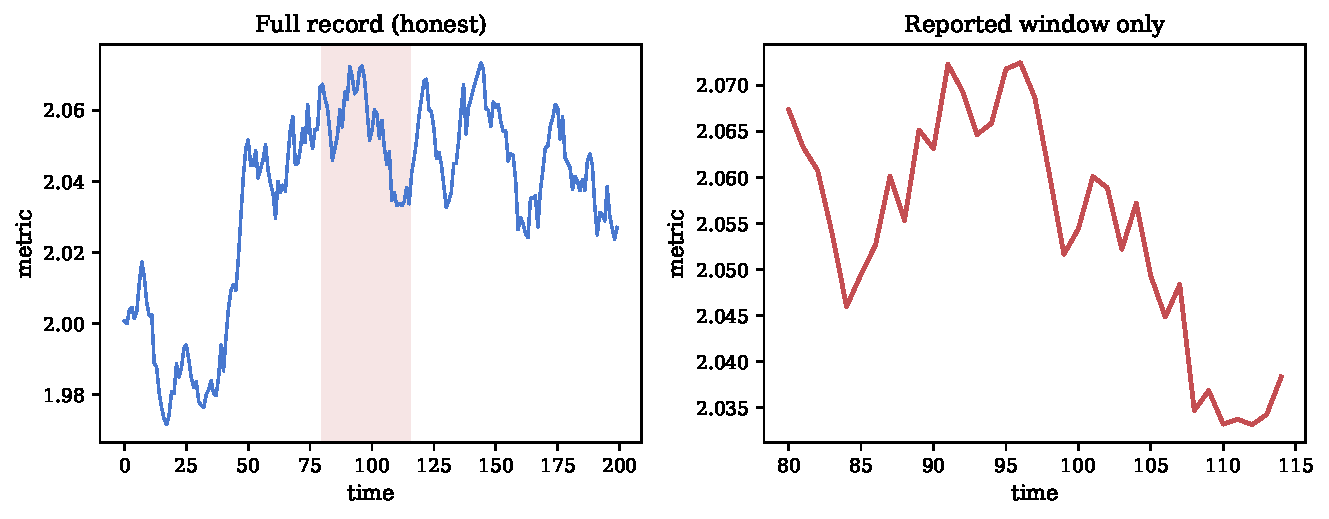
\includegraphics[width=0.95\textwidth]{imgs/cherry_time.pdf}
\end{figure}


\end{frame}

\begin{frame}[fragile]
\frametitle{Omitting Uncertainty}
\begin{figure}
\centering
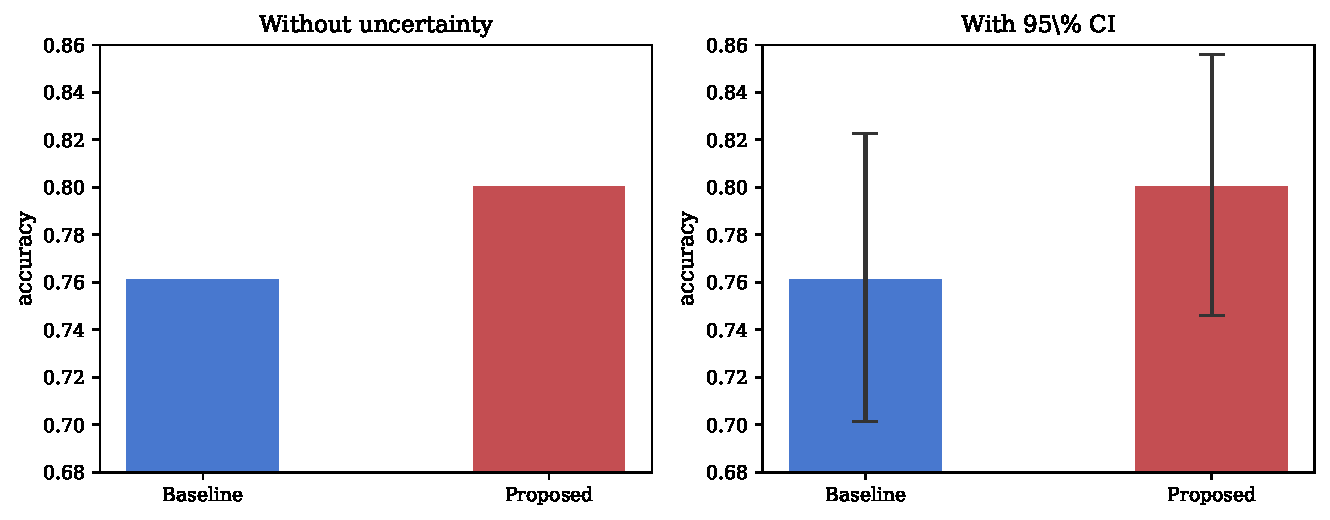
\includegraphics[width=0.95\textwidth]{imgs/error_bars.pdf}
\end{figure}


\end{frame}

\begin{frame}[fragile]
\frametitle{Over-Smoothing}
\begin{figure}
\centering
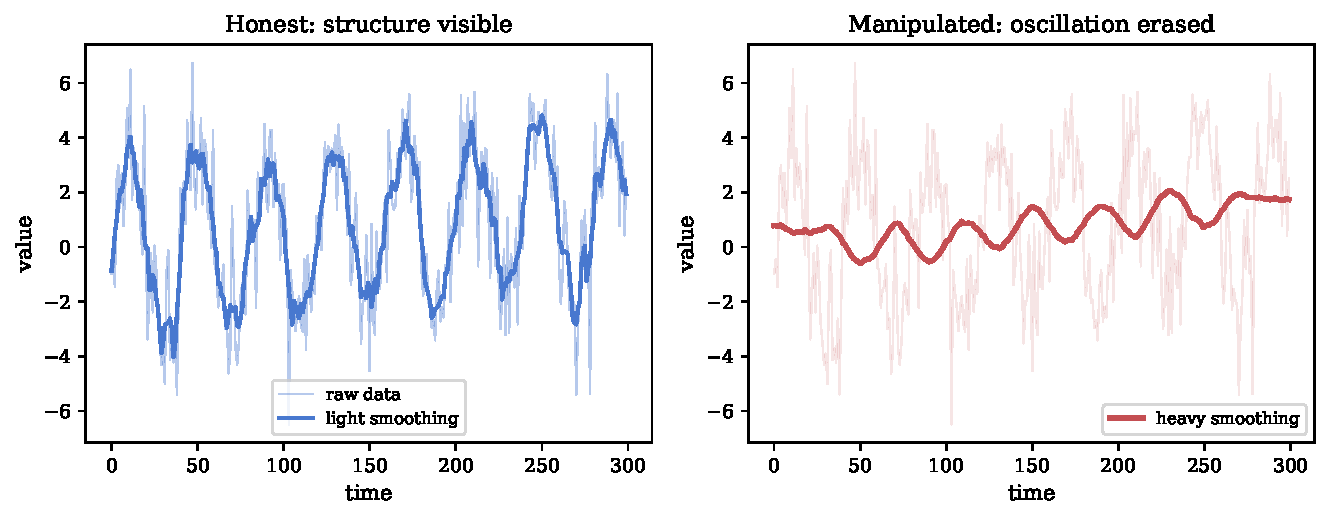
\includegraphics[width=0.95\textwidth]{imgs/smoothing.pdf}
\end{figure}


\end{frame}

\begin{frame}[fragile]
\frametitle{Aspect Ratio Manipulation}
\begin{figure}
\centering
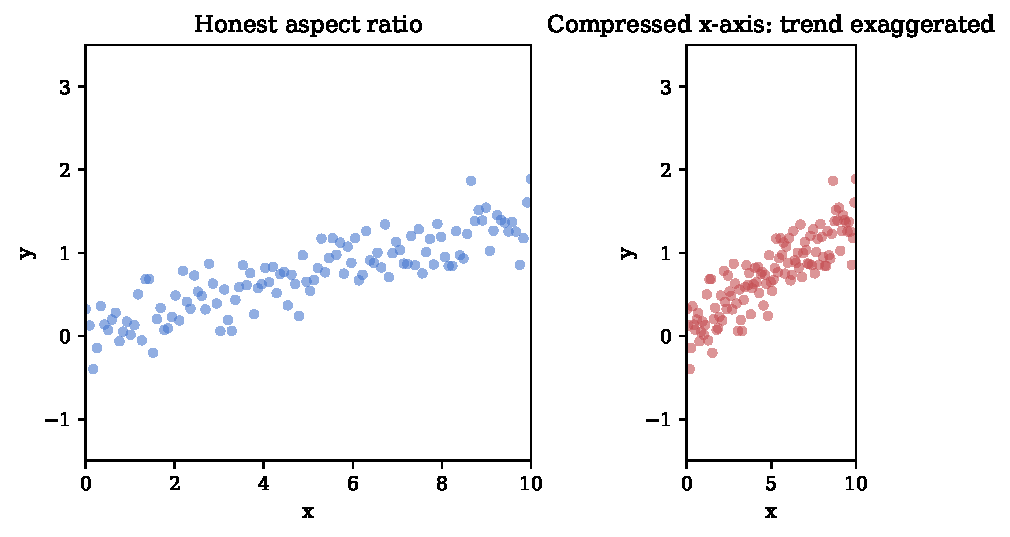
\includegraphics[width=0.95\textwidth]{imgs/aspect_ratio.pdf}
\end{figure}


\end{frame}

\section{Machine Learning–Specific Issues}

\begin{frame}[fragile]
\frametitle{Test Set Contamination}
\textbf{Contamination}: test information leaks into training or model selection.

Forms:
\begin{itemize}
  \item test samples included in the training set (data leakage);
  \item preprocessing statistics (mean, variance) computed over the full dataset;
  \item future information leaks into the past in time-series settings.
\end{itemize}

\end{frame}

\begin{frame}[fragile]
\frametitle{Leaderboard Overfitting}
\begin{figure}
\centering
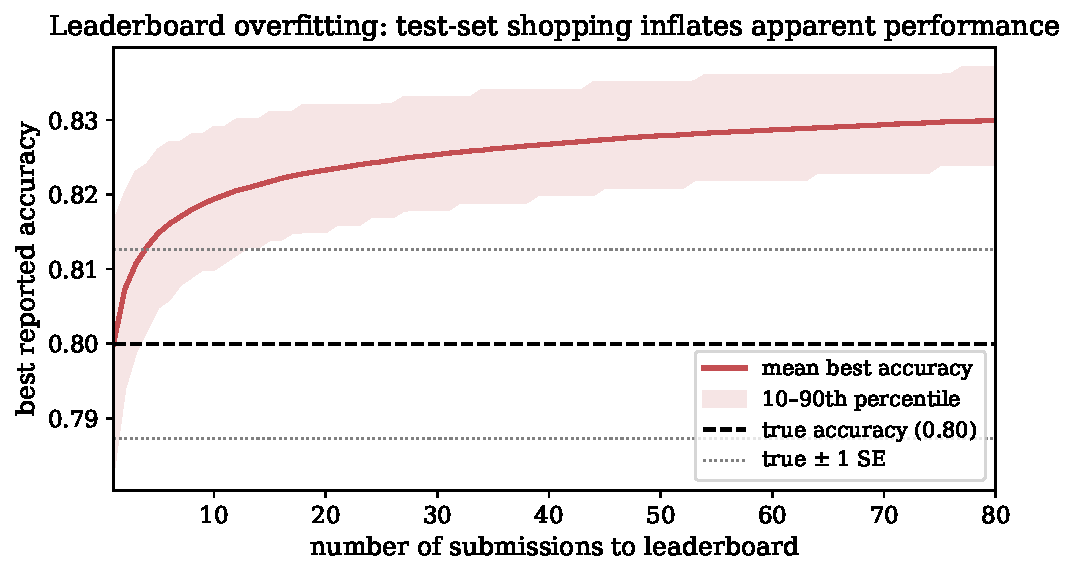
\includegraphics[width=0.9\textwidth]{imgs/leaderboard.pdf}
\end{figure}


{\small Repeated evaluation against a fixed test set inflates best-so-far accuracy even when no model improves. True accuracy (dashed) is constant.}

\end{frame}

\begin{frame}[fragile]
\frametitle{Leaderboard Overfitting: Analysis}
$k$ submissions, true accuracy $p$, test set size $n$, $\sigma = \sqrt{p(1-p)/n}$:

$$\mathbb{E}\!\left[\max_{i \leq k} \hat{p}_i\right] \approx p + \sigma \cdot \Phi^{-1}\!\!\left(\frac{k}{k+1}\right)$$

$n = 1000$, $p = 0.80$, $k = 80$:
\begin{itemize}
  \item best-reported accuracy $\approx 0.815$.
\end{itemize}

\end{frame}

\begin{frame}[fragile]
\frametitle{Benchmark Gaming}
\begin{itemize}
  \item \textbf{dataset-specific tuning}: hyperparameters optimised for the benchmark, not by cross-validation;
  \item \textbf{metric shopping}: report only the metric where the method ranks first;
  \item \textbf{benchmark construction bias}: benchmark designed to favour properties of one's own method;
  \item \textbf{selective comparison}: omit concurrent work that would narrow the gap.
\end{itemize}

\end{frame}

\begin{frame}[fragile]
\frametitle{Reproducibility in ML}
Pineau et al.\ (2021): a substantial fraction of ML papers do not release code, do not specify seeds, do not report variance, do not document hardware.

Henderson et al.\ (2018): deep RL results vary by up to 300\% across seeds and implementation details — never disclosed in the original papers.

\end{frame}

\section{Publication Malpractice}

\begin{frame}[fragile]
\frametitle{Salami Slicing}
\textbf{Salami slicing}: dividing one body of work into multiple minimal publications.

\begin{itemize}
  \item inflates publication count without proportional contribution;
  \item fragments the record — reviewers cannot see the full picture.
\end{itemize}

\end{frame}

\begin{frame}[fragile]
\frametitle{Duplicate Publication}
\textbf{Duplicate publication}: same work submitted to multiple venues without disclosure.

Legitimate:
\begin{itemize}
  \item conference $\to$ journal with substantial extension (disclosed);
  \item preprint $\to$ peer-reviewed venue (standard practice).
\end{itemize}

Not legitimate: simultaneous submission, superficial repackaging without disclosure.

\end{frame}

\begin{frame}[fragile]
\frametitle{Authorship Fraud}
ICMJE criteria: each author must have made a substantial intellectual contribution, participated in drafting, approved the final version, and be accountable.

Violations:
\begin{itemize}
  \item \textbf{gift authorship}: non-contributors added for prestige;
  \item \textbf{ghost authorship}: real contributors omitted (common in industry-funded trials);
  \item \textbf{coercive authorship}: authorship demanded in exchange for resources.
\end{itemize}

\end{frame}

\section{The Replication Crisis}

\begin{frame}[fragile]
\frametitle{Scale of the Problem}
{\footnotesize
\begin{tabular}{p{5.5cm} r p{3.5cm}}
\toprule
\textbf{Study} & \textbf{Rate} & \textbf{Field} \\
\midrule
Open Science Collaboration (2015) & 36–39\% & Psychology \\
Camerer et al.\ (2018) & 62\% & Economics \\
Begley \& Ellis (2012) & 11\% & Cancer biology \\
Reprod.\ Project: Cancer Biology (2021) & 50\% & Cancer biology \\
\bottomrule
\end{tabular}
}

\end{frame}

\begin{frame}[fragile]
\frametitle{Structural Causes}
The crisis is driven by incentives, not primarily by fraud:
\begin{itemize}
  \item \textbf{publication bias}: positive results published; null results filed away;
  \item \textbf{underpowered studies}: small $n$ inflates estimates conditional on significance;
  \item \textbf{researcher degrees of freedom}: legitimate choices collectively inflate false positive rate;
  \item \textbf{career incentives}: novel positive results rewarded; replications are not.
\end{itemize}

\end{frame}

\begin{frame}[fragile]
\frametitle{The Winner's Curse}
Conditioning on $p < \alpha$ in an underpowered study ($1 - \beta \ll 1$):

$$\mathbb{E}[\hat{\delta} \mid p < \alpha] > \delta_{\text{true}}$$

Published estimates are biased upward. Adequately powered replications find smaller effects — the published literature is a biased sample of all studies conducted.

\end{frame}

\section{Safeguards}

\begin{frame}[fragile]
\frametitle{Registered Reports}
\textbf{Registered Reports}: peer review before data collection; acceptance contingent on question and method, not outcome.

{\footnotesize
\begin{tabular}{p{4.5cm} p{4.5cm}}
\toprule
\textbf{Standard} & \textbf{Registered Report} \\
\midrule
Idea $\to$ Data $\to$ Paper $\to$ Review & Idea $\to$ Review $\to$ Data $\to$ Paper \\
\addlinespace
Acceptance depends on results & Acceptance independent of results \\
\addlinespace
Publication bias acts & Publication bias structurally eliminated \\
\bottomrule
\end{tabular}
}

\end{frame}

\begin{frame}[fragile]
\frametitle{Open Data and Code}
\begin{itemize}
  \item enables independent verification;
  \item allows error detection before findings propagate;
  \item makes the methods section verifiable, not merely aspirational.
\end{itemize}

\end{frame}

\begin{frame}[fragile]
\frametitle{Practical Checklist}
\textbf{Statistics:}
\begin{itemize}
  \item pre-specify primary outcome and analysis plan;
  \item apply multiple comparison corrections;
  \item report all outcomes.
\end{itemize}

\textbf{Machine learning:}
\begin{itemize}
  \item fix splits before any modelling decision;
  \item multiple seeds (5-10); compute estimate errors;
  \item tune all baselines equally;
  \item release code.
\end{itemize}

\end{frame}

\begin{frame}[fragile]
\frametitle{Recognising QRPs in the Wild}
When reading a paper:
\begin{itemize}
  \item are baselines recent and competitively tuned?
  \item are null or negative results present?
  \item is the method section sufficient for reimplementation?
  \item \textbf{are estimate errors reported?}
\end{itemize}

\end{frame}

\section{Conclusion}

\begin{frame}[fragile]
\frametitle{Summary}
{\footnotesize
\begin{tabular}{p{3.5cm} p{6cm}}
\toprule
\textbf{Category} & \textbf{Examples} \\
\midrule
Misconduct (FFP) & Fabrication, falsification, plagiarism \\
\addlinespace
Statistical QRPs & $p$-hacking, HARKing, optional stopping, outcome switching \\
\addlinespace
Methodological QRPs & Cherry-picking, inappropriate baselines, benchmark gaming \\
\addlinespace
Publication QRPs & Salami slicing, gift authorship, duplicate publication \\
\addlinespace
ML-specific QRPs & Leaderboard overfitting, test contamination, metric shopping \\
\midrule
Safeguards & Pre-registration, open data/code, registered reports \\
\bottomrule
\end{tabular}
}

\end{frame}

\section{References}

\begin{frame}[fragile]
\frametitle{References 1}
{\scriptsize
\begin{itemize}
\setlength\itemsep{0.25em}
\item Begley \& Ellis (2012). Raise standards for preclinical cancer research. \textit{Nature}, 483, 531--533.
\item Camerer et al.\ (2018). Replicability of social science experiments in \textit{Nature} and \textit{Science}. \textit{Nat.\ Hum.\ Behav.}, 2, 637--644.
\item Chan et al.\ (2004). Selective reporting of outcomes in randomized trials. \textit{JAMA}, 291, 2457--2465.
\item Errington et al.\ (2021). Investigating the replicability of preclinical cancer biology. \textit{eLife}, 10, e71601.
\item Gelman \& Loken (2014). The statistical crisis in science. \textit{Am.\ Scientist}, 102, 460--465.
\item Ioannidis, J.P.A.\ (2005). Why most published research findings are false. \textit{PLOS Med.}, 2(8), e124.
\item Henderson et al.\ (2018). Deep reinforcement learning that matters. \textit{AAAI}, 3207--3214.
\item Kerr (1998). HARKing: Hypothesizing after the results are known. \textit{PSPR}, 2, 196--217.
\end{itemize}
}

\end{frame}

\begin{frame}[fragile]
\frametitle{References 2}
{\scriptsize
\begin{itemize}
\setlength\itemsep{0.25em}
\item Open Science Collaboration (2015). Reproducibility of psychological science. \textit{Science}, 349, aac4716.
\item Pineau et al.\ (2021). Improving reproducibility in machine learning research. \textit{JMLR}, 22(164), 1--20.
\item Ahmed, A.M. et al.\ (2026). Extracting books from production language models. ArXiv, abs/2601.02671.
\item Huang, J. et al.\ (2024). Demystifying Verbatim Memorization in Large Language Models. EMNLP 2024
\end{itemize}
}
\end{frame}




\end{document}
